\documentclass[10pt]{article}

\usepackage{spheric}
%%%TITLE
\title{Aircraft tire water spray simulation using SPH}
\date{}


%%AFFILIATIONS
\author[1]{Yongkang HU$^\dagger$}
\author[1]{Yingfei RONG}
\author[1]{Dexin LENG}
\affil[1]{Triangle Tire R\&D, China}

\author[2]{Fei XU}
\author[2]{Xiangyang GAO}
\affil[2]{Northwest Polytechnical University, China}

\author[3]{Rengang CAO}
\author[3]{Wei DING}
\author[3]{Jun LV}
\affil[3]{COMAC, China}

\affil[$\relax$]{\email{\dagger}{huyongkang@triangle.com.cn}}


%%DOCUMENT
\begin{document}

\maketitle

%\SelectedTopics{}

%%PLEASE PUT YOUR ABSTRACT HERE
\begin{abstract}
The sprays produced by aircraft tire running in water are complex and depends on the aircraft speed, tire shape and load, also the water depth. The serious consequence of water spray ingestion is the loss of engine power which will impact on the take-off and landing operations.

The present paper aims to investigate the chine design parameters of aircraft tire in function of water spray performance. Detailed aircraft tire construction models are being built with different chine design parameters using Abaqus/Explicit. The interaction between the aircraft and water is modeled using general contact of SPH elements on tire structure elements.

The numerical simulations at different loading and aircraft speeds are performed with different chine design models. Figure below illustrates clearly the impact of chine shape on water spray pattern, position and speed. 

\begin{figure}[!htb]
\centering
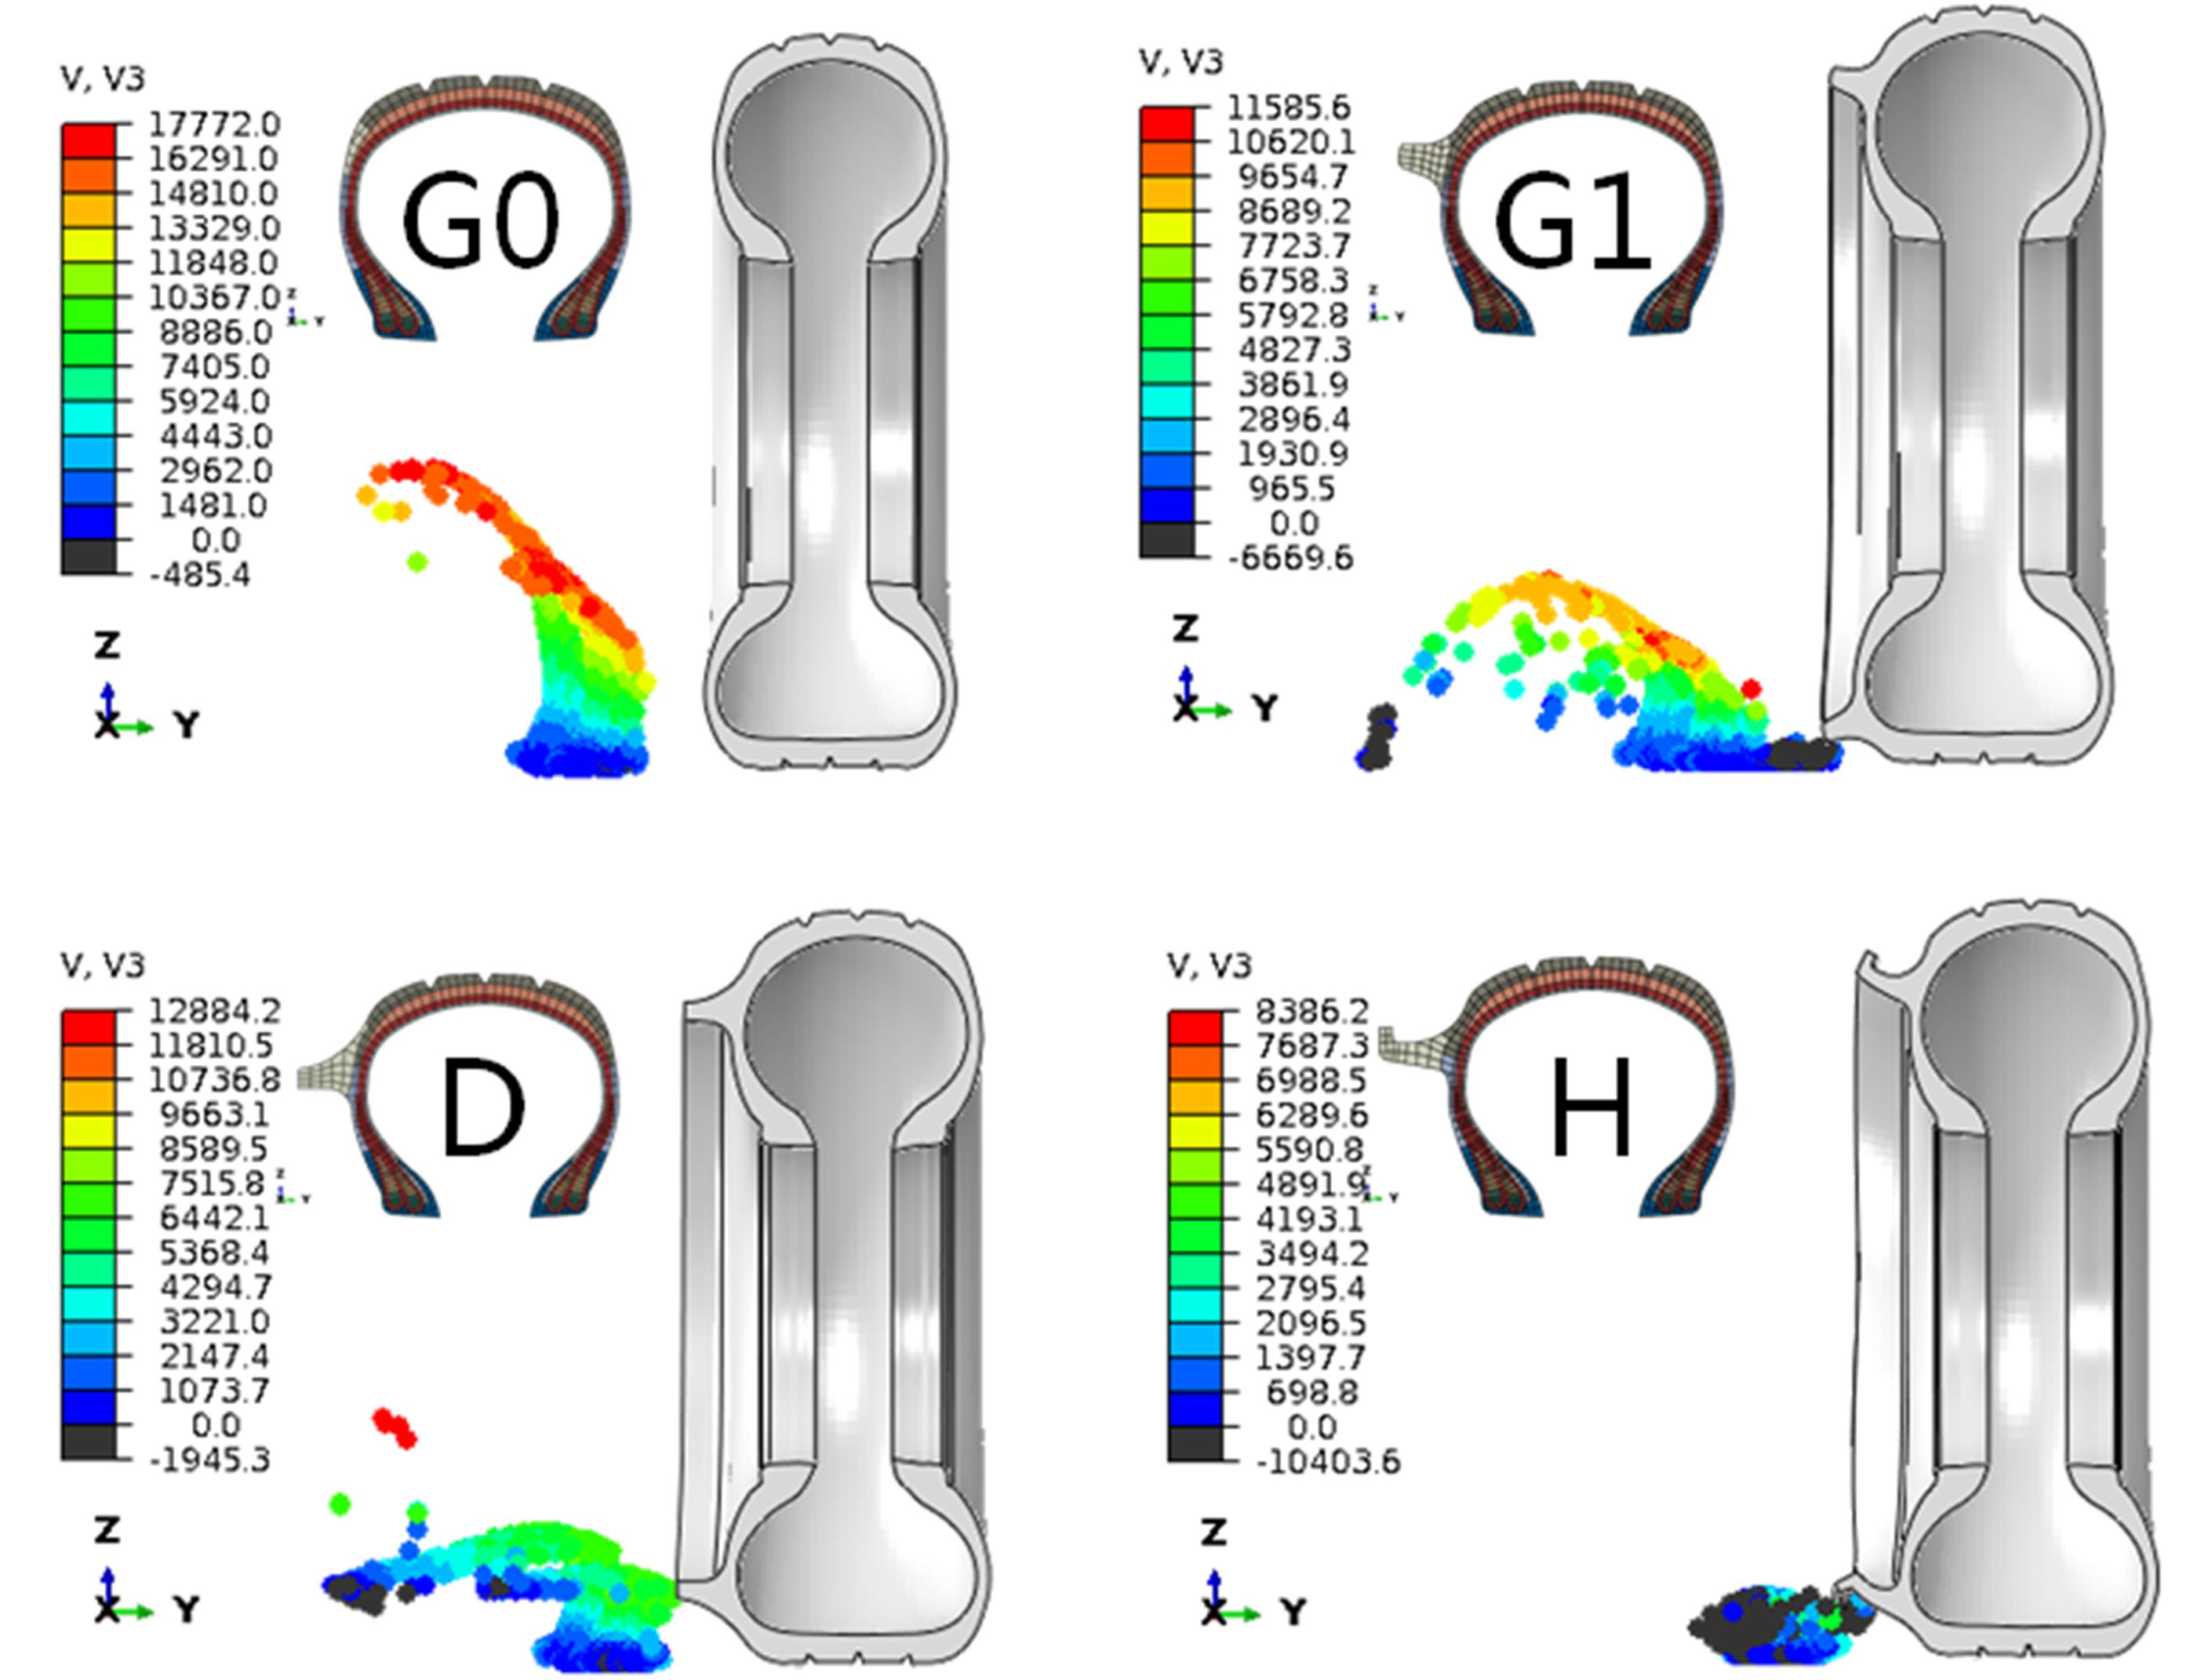
\includegraphics[width=0.75\textwidth]{30-1.png}
\caption{water spray pattern at 90 knots (Loads = 22266.4 N, Pressure = 0.869 MPa)}\label{fig:30}
\end{figure}

\end{abstract}


%%THE END OF ABSTRACT

\addbib

\end{document}
